% =============================================================================
%  fig_confidence_framework.tex
%  Confidence score computation framework — four sub-scores → weighted sum
% =============================================================================
\documentclass[tikz, border=6pt]{standalone}
\usepackage{tikz}
\usepackage{amsmath}
\usetikzlibrary{shapes.geometric, shapes.misc, arrows.meta, positioning,
                fit, backgrounds, calc}

\definecolor{rC}  {RGB}{31, 119, 180}
\definecolor{cC}  {RGB}{255, 127,  14}
\definecolor{bC}  {RGB}{ 44, 160,  44}
\definecolor{pC}  {RGB}{148, 103, 189}
\definecolor{gC}  {RGB}{ 80,  80,  80}

\tikzset{
  inp/.style  = {rectangle, rounded corners=2pt, draw=#1, fill=#1!12,
                 line width=0.8pt, text width=2.8cm, align=center,
                 minimum height=1.0cm, font=\footnotesize},
  score/.style= {rectangle, rounded corners=2pt, draw=#1, fill=#1!20,
                 line width=0.7pt, text width=2.2cm, align=center,
                 minimum height=0.8cm, font=\footnotesize},
  wt/.style   = {circle, draw=gray!70, fill=white, line width=0.7pt,
                 font=\scriptsize, inner sep=2pt, minimum size=0.7cm},
  sigma/.style= {circle, draw=gC, fill=gC!15, line width=1.0pt,
                 font=\normalsize\bfseries, inner sep=4pt, minimum size=1.2cm},
  outbox/.style= {rectangle, rounded corners=3pt, draw=gC, fill=gC!10,
                 line width=1.0pt, text width=2.8cm, align=center,
                 minimum height=1.0cm, font=\small\bfseries},
  dec/.style  = {diamond, aspect=2.2, draw=red!70, fill=red!8, line width=0.8pt,
                 align=center, font=\footnotesize, inner sep=2pt},
  arr/.style  = {-{Stealth[length=4pt]}, line width=0.8pt, color=gray!70!black},
  lbl/.style  = {font=\scriptsize, color=gray!60!black},
}

\begin{document}
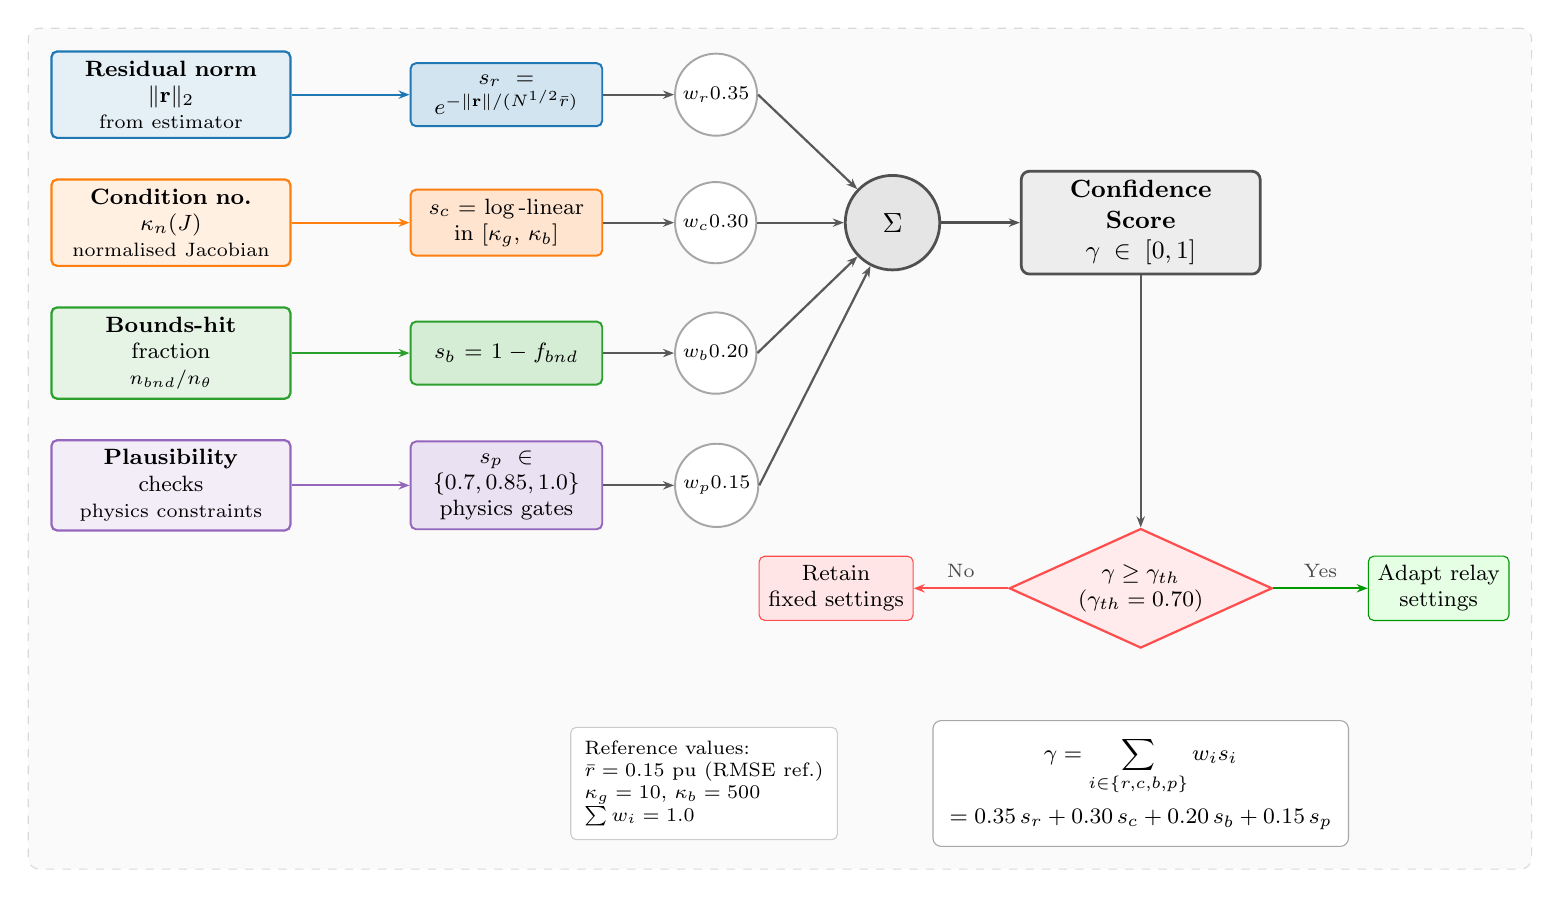
\begin{tikzpicture}[node distance=0.5cm and 1.1cm]

% ---- Input column -----------------------------------------------------------
\node[inp=rC] (ir) {%
  \textbf{Residual norm}\\$\|\mathbf{r}\|_2$\\
  \scriptsize from estimator};

\node[inp=cC, below=of ir] (kj) {%
  \textbf{Condition no.}\\$\kappa_n(J)$\\
  \scriptsize normalised Jacobian};

\node[inp=bC, below=of kj] (bh) {%
  \textbf{Bounds-hit}\\fraction\\
  \scriptsize $n_{bnd}/n_\theta$};

\node[inp=pC, below=of bh] (pp) {%
  \textbf{Plausibility}\\checks\\
  \scriptsize physics constraints};

% ---- Score column -----------------------------------------------------------
\node[score=rC, right=1.5cm of ir] (sr) {%
  $s_r = e^{-\|\mathbf{r}\|/(N^{1/2}\bar{r})}$};

\node[score=cC, right=1.5cm of kj] (sc) {%
  $s_c = \log\text{-linear}$\\in $[\kappa_g,\,\kappa_b]$};

\node[score=bC, right=1.5cm of bh] (sb) {%
  $s_b = 1 - f_{bnd}$};

\node[score=pC, right=1.5cm of pp] (sp) {%
  $s_p \in \{0.7, 0.85, 1.0\}$\\physics gates};

% ---- Arrows: input → score --------------------------------------------------
\draw[arr, color=rC] (ir.east) -- (sr.west);
\draw[arr, color=cC] (kj.east) -- (sc.west);
\draw[arr, color=bC] (bh.east) -- (sb.west);
\draw[arr, color=pC] (pp.east) -- (sp.west);

% ---- Weight column ----------------------------------------------------------
\node[wt, right=0.9cm of sr] (wr) {$w_r$\\$0.35$};
\node[wt, right=0.9cm of sc] (wc) {$w_c$\\$0.30$};
\node[wt, right=0.9cm of sb] (wb) {$w_b$\\$0.20$};
\node[wt, right=0.9cm of sp] (wp) {$w_p$\\$0.15$};

\draw[arr] (sr.east) -- (wr.west);
\draw[arr] (sc.east) -- (wc.west);
\draw[arr] (sb.east) -- (wb.west);
\draw[arr] (sp.east) -- (wp.west);

% ---- Summation node ---------------------------------------------------------
\node[sigma, right=1.1cm of wc] (sum) {$\Sigma$};

\foreach \w in {wr, wc, wb, wp}
  \draw[arr] (\w.east) -- (sum);

% ---- Output: gamma ----------------------------------------------------------
\node[outbox, right=1.0cm of sum] (gam) {%
  Confidence\\Score\\$\gamma \in [0,1]$};

\draw[arr, line width=1.1pt, color=gC] (sum) -- (gam);

% ---- Decision gate ----------------------------------------------------------
% Directly below gam — straight vertical arrow, clears all input rows
\node[dec, below=3.2cm of gam] (dec) {$\gamma \geq \gamma_{th}$\\$(\gamma_{th}=0.70)$};

\draw[arr] (gam.south) -- (dec.north);

\node[rectangle, rounded corners=2pt, draw=green!60!black, fill=green!10,
      align=center, font=\footnotesize, right=1.2cm of dec]
      (yes) {Adapt relay\\settings};

\node[rectangle, rounded corners=2pt, draw=red!70, fill=red!10,
      align=center, font=\footnotesize, left=1.2cm of dec]
      (no)  {Retain\\fixed settings};

\draw[arr, color=green!60!black] (dec.east) -- node[lbl, above]{Yes} (yes.west);
\draw[arr, color=red!70]         (dec.west) -- node[lbl, above]{No}  (no.east);

% ---- Equation box -----------------------------------------------------------
% Below the decision diamond, centred
\node[draw=gC!50, fill=white, rounded corners=3pt, inner sep=6pt,
      align=center, font=\footnotesize, below=0.9cm of dec]
  (eqbox)
{$\gamma = \displaystyle\sum_{i\in\{r,c,b,p\}} w_i s_i$\\[4pt]
 $= 0.35\,s_r + 0.30\,s_c + 0.20\,s_b + 0.15\,s_p$};

% ---- Score normalisation annotation -----------------------------------------
\node[draw=gray!40, fill=white, rounded corners=2pt, inner sep=5pt,
      align=left, font=\scriptsize, left=1.2cm of eqbox]
  (refbox)
{Reference values:\\
 $\bar{r}=0.15$ pu (RMSE ref.)\\
 $\kappa_g = 10$, $\kappa_b = 500$\\
 $\sum w_i = 1.0$};

% ---- Background groups ------------------------------------------------------
\begin{scope}[on background layer]
  \node[rectangle, rounded corners=4pt, draw=gray!30, fill=gray!4,
        dashed, inner sep=8pt,
        fit=(ir)(kj)(bh)(pp)(sr)(sc)(sb)(sp)(wr)(wc)(wb)(wp)(sum)(gam)
            (dec)(yes)(no)(eqbox)(refbox)] {};
\end{scope}

\end{tikzpicture}
\end{document}
